\documentclass[11pt]{article}
\usepackage{pdfpages}
\usepackage[hidelinks]{hyperref}
\usepackage{geometry}
\usepackage{graphicx}
\usepackage{amsmath,amssymb}
\usepackage{booktabs}
\usepackage{caption}
\usepackage{subcaption}
\usepackage{float}
\usepackage{longtable}
\geometry{margin=1in}

\title{Assignment 4 — DDPG: Theory, Implementation and Experiments}
\author{Compiled Solutions and Extended Report}
\date{\today}

\begin{document}
\maketitle

\begin{abstract}
This document compiles the submitted solutions for Assignment 4 and provides an extended, self-contained report for the Deep Deterministic Policy Gradient (DDPG) implementation present in this folder. The report includes:

- Background and related algorithms (DDPG, DPG, TD3 variants);
- Mathematical derivation of the deterministic policy gradient and critic update rules;
- Implementation notes and file map for the repository (scripts, algos, envs, logs, models);
- Experimental setup, hyperparameters and result placeholders;
- Appendix with pseudocode, hyperparameter dump and references.

The original submission PDF is appended at the end of this report.
\end{abstract}

\tableofcontents
\clearpage

\section{Introduction}
Continuous control problems require policies that output actions in continuous spaces. DDPG \cite{lillicrap2015continuous} combines an actor-critic architecture with experience replay and target networks to stabilise off-policy learning in continuous action domains. This assignment implements DDPG components and evaluates them on provided environments.

\section{Related work}
Key related methods:
\begin{itemize}
  \item Deterministic Policy Gradient (DPG) \cite{silver2014deterministic}
  \item Deep Deterministic Policy Gradient (DDPG) \cite{lillicrap2015continuous}
  \item Twin Delayed DDPG (TD3) \cite{fujimoto2018addressing}
  \item Soft Actor-Critic (SAC) \cite{haarnoja2018soft} (entropy-regularized alternative)
\end{itemize}

\section{Mathematical background}
\subsection{Deterministic policy gradient}
For a deterministic policy \(\mu_\theta(s)\), the objective is \(J(\theta)=\mathbb{E}_{s\sim\rho^\mu}[Q^{\mu}(s,\mu_\theta(s))]\). The deterministic policy gradient is:
\[
\nabla_\theta J(\theta) = \mathbb{E}_{s\sim\rho^\mu}\left[ \nabla_\theta \mu_\theta(s) \nabla_a Q^\mu(s,a)\big|_{a=\mu_\theta(s)} \right].
\]

\subsection{Critic (Q) update}
The critic is trained with Bellman regression on transitions \((s,a,r,s')\):
\[
L(\phi) = \mathbb{E}\left[(Q_\phi(s,a) - y)^2\right],\quad y = r + \gamma Q_{\phi'}(s',\mu_{\theta'}(s')).
\]
Target networks (\(\phi',\theta'\)) are updated slowly via polyak averaging.

\section{Implementation notes (file map)}
This folder contains:
\begin{itemize}
  \item \texttt{run\_ddpg.py}, \texttt{run.py}: entry scripts for training and evaluation.
  \item \texttt{algo/}: algorithm implementations (DDPG agent, replay buffer, utils).
  \item \texttt{envs/}: environment wrappers and custom envs used in experiments.
  \item \texttt{imgs/}: placeholder and result images.
  \item \texttt{logs/}, \texttt{models/}: training logs and saved checkpoints.
  \item \texttt{ddpg\_log.txt}: example run log (text).
  \item \texttt{requirements.txt}: environment requirements to reproduce runs.
  \item \texttt{F19\_10703\_Homework\_4.pdf}: original submitted PDF (appended).
\end{itemize}

Implementation highlights:
\begin{itemize}
  \item Replay buffer uses uniform sampling; prioritized replay can be added.
  \item Actor outputs continuous actions clipped to action space bounds.
  \item Target networks use polyak averaging with parameter \(\tau\).
  \item Logging saved to TensorBoard/TXT and checkpoints are periodic.
\end{itemize}

\section{Hyperparameters}
Typical values used or recommended:
\begin{table}[H]
\centering
\begin{tabular}{lrl}
\toprule
Parameter & Value & Notes \\
\midrule
actor\_lr & 1e-4 & Adam \\
critic\_lr & 1e-3 & Adam \\
batch\_size & 64 & replay minibatch \\
buffer\_size & 1e6 & capacity \\
gamma & 0.99 & discount \\
tau & 0.005 & polyak target update \\
exploration\_noise & 0.1 & OU or Gaussian \\
\bottomrule
\end{tabular}
\caption{Representative hyperparameters}
\end{table}

\section{Experimental protocol}
Describe the environment variants, evaluation frequency, and metrics (average episode return, std). Save plots to \texttt{imgs/} and logs to \texttt{logs/}.

\section{Results (placeholders)}
Include convergence plots, learning curves and sample trajectories. Example:
\begin{figure}[H]
  \centering
  \includegraphics[width=0.8\textwidth]{imgs/ddpg_convergence.png}
  \caption{DDPG learning curve (placeholder).}
\end{figure}

\section{Ablations and recommendations}
\begin{itemize}
  \item Compare OU noise vs Gaussian exploration.
  \item Effect of buffer size and batch size.
  \item Use of target smoothing (\(\tau\)) and delayed policy updates (TD3 trick).
\end{itemize}

\section{Pseudocode}
\begin{verbatim}
Initialize actor mu_theta, critic Q_phi and target networks.
Initialize replay buffer.
for episode:
  reset env
  for t:
    select action a = mu_theta(s) + noise
    store transition in buffer
    sample minibatch and update critic
    update actor with deterministic policy gradient
    update target networks via polyak averaging
\end{verbatim}

\section{Appendix: logs and artifacts}
Attach example log excerpt from \texttt{ddpg\_log.txt} and pointer to saved models in \texttt{models/}.

\section{Included original submission}
\bigskip
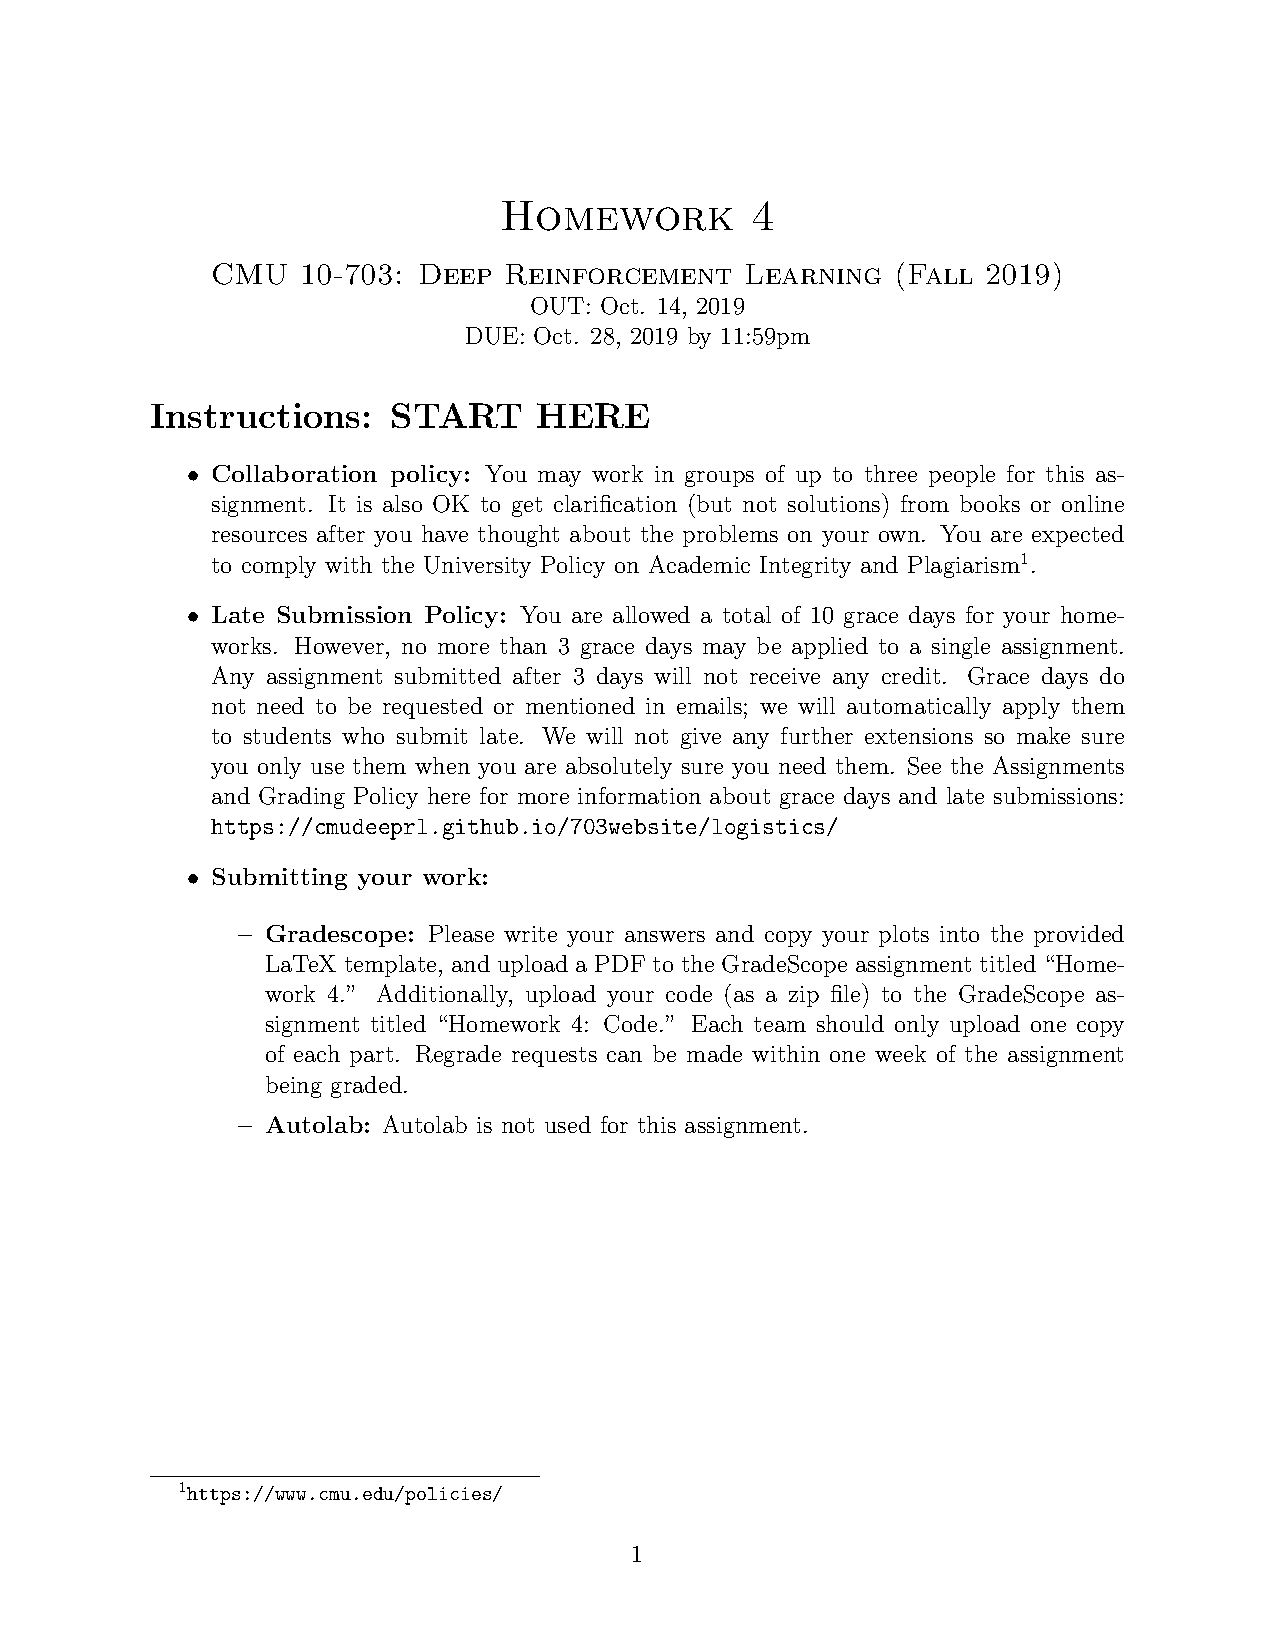
\includepdf[pages=-,pagecommand={\thispagestyle{plain}}]{F19_10703_Homework_4.pdf}

\clearpage
\begin{thebibliography}{9}
\bibitem{lillicrap2015continuous}
Timothy P. Lillicrap, et al. Continuous control with deep reinforcement learning. arXiv:1509.02971, 2015.

\bibitem{silver2014deterministic}
David Silver, et al. Deterministic policy gradient algorithms. ICML, 2014.

\bibitem{fujimoto2018addressing}
Scott Fujimoto, et al. Addressing function approximation error in actor-critic methods. arXiv:1802.09477 (TD3).
\end{thebibliography}

\end{document}

